\documentclass[11pt,a4paper,english,greek,twoside]{../Thesis}
\usepackage{amsmath}
\begin{document}
\chapter{Σημασιολογικό Υποσύστημα: Ο Τύπος Λαβής}
Ο τύπος λαβής (grasping type) είναι πρακτικά ο τρόπος με τον οποίο ένας άνθρωπος πιάνει ένα αντικείμενο με τα χέρια του προκειμένου να προβεί σε κάποια ενέργεια. Στην αναγνώριση δράσεων, μπορούμε να εξάγουμε χρήσιμες πληροφορίες από τον τύπο λαβής, τόσο για τον τύπο της δράσης, όσο και για τα όρια μιας δράσης. Από την πλευρά του συστήματος που θα δράσει μετά την αναγνώριση, ανθρώπου ή ρομπότ, ο τύπος λαβής είναι απαραίτητη πληροφορία για την αλληλεπίδραση με τα αντικείμενα.

\begin{figure}
  \centering
  \noindent\makebox[\textwidth]{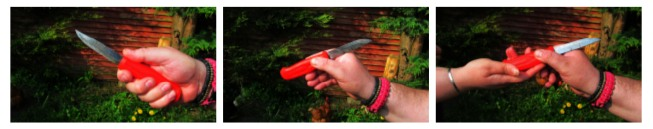
\includegraphics[scale=0.5]{{Images/chap5Intention}.jpg}}
  \caption{Ο σχηματισμός των χεριών στο χειρισμό των αντικειμένων εμπεριέχει σημασιολογική πληροφορία η οποία μπορεί να υποδεικνύει την πρόθεση ή τη δράση αυτή καθαυτή. Στην εικόνα αριστερά γα παράδειγμα, ο τρόπος λαβής του μαχαιριού είναι προσανατολισμένος στη δύναμη και μπορούμε να υποθέσουμε ότι το μαχαίρι πρόκειται να χρησιμοποιηθεί σε κάποια εργασία. Αντίθετα στη μεσαία εικόνα, ο τύπος λαβής είναι προσανατολισμένος στην ακρίβεια. Η φυσική απόκριση στη λαβή αυτή είναι να δεχτούμε το μαχαίρι που μας αποδίδεται, όπως στην εικόνα δεξιά. Εικόνα από \cite{yang_2015_grasp}.}
  \label{fig:chap5Intention}
\end{figure}

\par Στη βιβλιογραφία εμφανίζονται ποικίλες μορφές τύπων λαβής, οι οποίες κατατάσσονται σε κατηγορίες ανάλογα με τα εκάστοτε κριτήρια \cite{feix_2013}. Από αυτές, τις ταξινομήσεις, η πιο χρήσιμη στην αναγνώριση δράσεων είναι η κατηγοριοποίηση με βάση τη λειτουργία, σε λαβές ακριβείας και δύναμης \cite{jeannerod_1984}.

\par Σε αυτή την εργασία, η προσέγγισή μας στην αναγνώριση τύπου λαβής εκκινεί με την ανίχνευση των χεριών του ανθρώπου-δράστη στο βίντεο. Συνεχίζουμε με την εκπαίδευση πάνω στις εικόνες χεριών για την εξαγωγή του τύπου λαβής με χρήση συνελικτικών χαρακτηριστικών και τελικά εξάγουμε τα ιστογράμματα τύπων λαβής για τα βίντεο των δεδομένων ελέγχου (test). Το κεφάλαιο οργανώνεται ως εξής: Πρώτα γίνεται μια αναφορά σε νευρωνικά δίκτυα και συνελικτικά χαρακτηριστικά. Στη συνέχεια παρουσιάζουμε τη μέθοδο ανίχνευσης χεριών και τα χαρακτηριστικά BING. Τελικά δείχνουμε τη σύζευξη όλων αυτών των μεθόδων με χρήση μη επιβλεπόμενης μάθησης για την εξαγωγή των ιστογραμμάτων τύπων λαβής.


\section{Θεωρητικό Υπόβαθρο}
\subsection{Νευρωνικά Δίκτυα}
Η ιδέα του νευρωνικού δικτύου εισάγεται για πρώτη φορά στα τέλη της δεκαετίας του '50 με τον περίφημο αλγόριθμο Perceptron \cite{rosenblatt_1958}. Ο αλγόριθμος στοχεύει στο να προσαρμόσει στα δεδομένα εκπαίδευσης έναν γραμμικό ταξινομητή έτσι ώστε να ελαχιστοποιήσει κάποιο κριτήριο κόστους που σχετίζεται με την ακρίβεια ταξινόμησης, “δείχνοντας” επαναλαμβανόμενα τα δείγματα εκπαίδευσης στον ταξινομητή. Αποδεικνύεται ότι ο αλγόριθμος Perceptron συγκλίνει και η δομική μονάδα αυτή, δηλαδή ο προκύπτων ταξινομητής, είναι ένας νευρώνας, δομικός λίθος ενός νευρωνικού δικτύου. Ωστόσο, η εμφάνιση ικανοποιητικών αποτελεσμάτων μετά τη σύγκλιση προϋποθέτει γραμμική διαχωρισιμότητα. Για επιπλέον διαχωρισμό του χώρου δεδομένων σε περιοχές, μπορούμε να συνδυάσουμε δομικές μονάδες Perceptron σε πολλαπλά επίπεδα. Αποδεικνύεται ότι με ένα νευρωνικό δίκτυο τριών επιπέδων μπορούμε να προσεγγίσουμε οποιαδήποτε συνάρτηση.

\begin{figure}
  \centering
  \noindent\makebox[\textwidth]{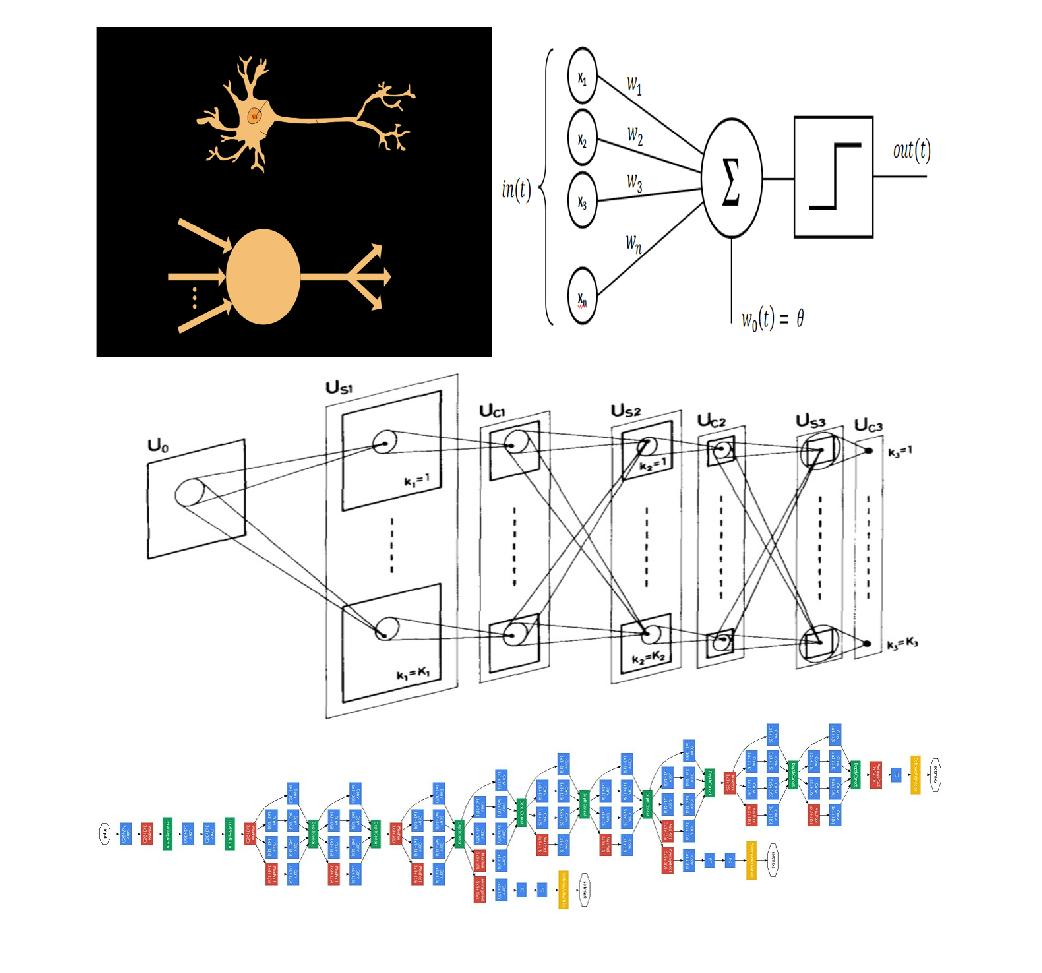
\includegraphics[scale=0.25]{{Images/chap5Neurals}.jpg}}
  \caption{Η εξέλιξη των νευρωνικών στην πορεία τους. Εκκινώντας εμπνεόμενα από τα βιολογικά νευρικά κύτταρα, τα πρώτα νευρωνικά δίκτυα αποτελούνταν από μια γραμμική συνδεσμολογία απλών νευρώνων σε επίπεδα. Στο Neocognitron \cite{fukushima_1980} εμφανίζεται η οργάνωση σε επίπεδα με διαφορετικό συναπτικό πεδίο που απεικονίζεται σε διαφορετικά τμήματα εισόδου. Οι νευρώνες και κατά συνέπεια τα εκφραζόμενα χαρακτηριστικά αποκτούν μια τοπικότητα η φαίνεται να χρησιμεύει ιδιαίτερα στην ανάλυση εικόνων και βίντεο. Στα τελευταία χρόνια, η χρήση ταχύτερου υλικού (hardware) και η ανάπτυξη προγραμματιστικών τεχνικών (παραλληλία) επέτρεψαν τη σχεδίαση και εφαρμογή βαθιών συνελικτικών δικτύων, όπως το εικονιζόμενο GoogLeNet \cite{szegedy_2015}, τα οποία έγιναν ασυναγώνιστα σε πολλά πεδία της Μηχανικής Μάθησης.}
  \label{fig:chap5Neurals}
\end{figure}

\par Το 1980, εισάγονται για πρώτη φορά οι συνάψεις με τοπικότητα μέσω αυτοοργανούμενων χαρτών και τα δίκτυα γίνονται βαθύτερα. Το Neocognitron \cite{fukushima_1980}, αποτελεί την εξέλιξη του προκατόχου του \cite{fukushima_1975} και αποτελεί το πρώτο Συνελικτικό Νευρωνικό δίκτυο, επηρεασμένο δομικά από τον οπτικό φλοιό της γάτας \cite{hubel_1962}. Καθώς η τεχνολογία εξελίσσεται, προτείνονται διαφοροποιήσεις \cite{lecun_1998} και απλοποιήσεις των Συνελικτικών Δικτύων \cite{behnke_2003}, \cite{simard_2003} και δομικές αλλαγές \cite{ciresan_2011} με την τεχνολογία των καρτών γραφικών υπολογιστή (GPU) να συμβάλλει στην αποτελεσματική εκπαίδευση βαθιών δικτύων \cite{ciresan_2012}. Η επανάσταση των Συνελικτικών Νευρωνικών Δικτύων γίνεται το 2012 \cite{alexnet_2012} με το μοντέλο AlexNet να κερδίζει τον ετήσιο διαγωνισμό αναγνώρισης αντικειμένων ImageNet Challenge σημειώνοντας μεγάλη αύξηση του ποσοστού επιτυχίας και ανοίγοντας το δρόμο για νέα εκτεταμένη έρευνα στο πεδίο των Νευρωνικών Δικτύων. Τα τελευταία χρόνια, τα Συνελικτικά Νευρωνικά Δίκτυα έχουν εξελιχθεί σε δομή και βάθος, με ικανότητα να πετυχαίνουν πολύ υψηλές επιδόσεις αναγνώρισης και ταυτόχρονα να είναι εξαιρετικά γρήγορα \cite{zeiler_2013}, \cite{szegedy_2015}, \cite{he_2015}, \cite{donahue_2015}. Επιπλέον, συναντούν ευρεία εφαρμογή πέραν της ταξινόμησης όπως η συντακτική ανάλυση \cite{chen_2014_fast}, η περιγραφή εικόνων \cite{yang_2015_neural}, \cite{vinyals_2015}, η ανίχνευση αντικειμένων \cite{ren_2016} και η κατάτμηση εικόνων \cite{long_2016}, ενώ έχει αρχίσει και η χρήση τους απευθείας σε βίντεο \cite{karpathy_2014}.

\par Θα δούμε τώρα σε μεγαλύτερο βάθος τη δομή και τη λειτουργία των Συνελικτικών Νευρωνικών Δικτύων. Τα κλασσικά νευρωνικά δίκτυα είναι ένας χάρτης νευρώνων που ενώνονται με πολλαπλασιαστικές συνάψεις και οι παράμετροί τους (βάρη) προσαρμόζονται στη διαδικασία της εκπαίδευσης. Με αυτόν τον τρόπο, κάθε νευρώνας εκτελεί έναν γραμμικό μετασχηματισμό ακολουθούμενο από μια μη γραμμικότητα. Το συνολικό δίκτυο εκφράζει έναν διαφορικό μετασχηματισμό της εισόδου σε σκορ κλάσεων. Τα συνελικτικά δίκτυα διατηρούν τις παραπάνω ιδιότητες αλλά στηρίζονται στην υπόθεση ότι η είσοδος θα είναι εικόνα, οπότε ποικίλες χρήσιμες ιδιότητες μπορούν επιπλέον να ενσωματωθούν στη δομή τους. Αυτό οδηγεί σε αλλαγή της χωρικής διάταξης με αραιές συνδέσεις, οι οποίες απαιτούν λιγότερα βάρη. Έτσι τα συνελικτικά δίκτυα είναι πιο γρήγορα, πιο ακριβή και πιο εύρωστα.

\par Η πρώτη κύρια διαφορά των συνελικτικών από τα κλασσικά νευρωνικά δίκτυα είναι ότι κάθε επίπεδο είναι τώρα τρισδιάστατο και έχει πλάτος, μήκος και βάθος. Προφανώς το τελευταίο στάδιο είναι διάνυσμα με διάσταση ίση με τον αριθμό των κλάσεων. Η ακόλουθη εικόνα δείχνει ένα συνελικτικό δίκτυο και επισημειώνει τις διαστάσεις ενός συνελικτικού σταδίου:

\begin{figure}[H]
  \centering
  \noindent\makebox[\textwidth]{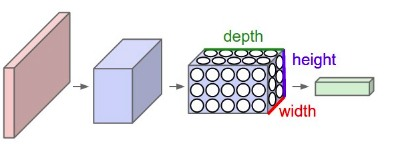
\includegraphics[scale=0.5]{{Images/chap5CNN1}.jpg}}
  \caption{Ένα συνελικτικό νευρωνικό δίκτυο οργανώνει τους νευρώνες του σε τρεις διαστάσεις, πλάτος, ύψος και βάθος, όπως οπτικοποιούνται εδώ σε ένα από τα επίπεδά του. Κάθε επίπεδο ενός συνελικτικού νευρωνικού δικτύου μετασχηματίζει έναν τρισδιάστατο όγκο εισόδου σε έναν τρισδιάτατο χώρο ενεργοποιήσεων νευρώνων.}
  \label{fig:chap5CNN1}
\end{figure}

\par Τα δίκτυα αυτά, αντίθετα με τα συμβατικά νευρωνικά, περιέχουν διάφορους τύπους σταδίων. Ο πιο βασικός είναι σίγουρα τα συνελικτικά στάδια, τα οποία είναι ο κύριος πυρήνας της εξαγωγής χαρακτηριστικών και υπολογίζουν την έξοδο νευρώνων που συνδέονται σε τοπικές περιοχές της εισόδου. Ακολουθούν τα pooling layers, τα οποία εκτελούν υποδειγματοληψία προκειμένου βαθμιαία να μειώνουν το μέγεθος των σταδίων και των παραμέτρων και να προστατεύουν από υπερπροσαρμογή (overfitting) και κόστος υπολογισμών. Συνήθως κοντά στο στάδιο εξόδου, τα συνελικτικά νευρωνικά δίκτυα περιέχουν κλασσικά, πλήρως συνδεδεμένα στάδια, όπως αυτά των κλασσικών νευρωνικών δικτύων, τα οποία παράγουν τα σκορ κλάσεων. Τέλος, μια κατηγορία σταδίων είναι τα ReLU (γραμμικοί περιοριστές), τα οποία είναι στην ουσία συναρτήσεις ενεργοποίησης που ακολουθούν τον υπολογισμό των συνελικτικών σταδίων, αντικαθιστώντας τις μη γραμμικές συναρτήσεις που χρησιμοποιούν τα συμβατικά νευρωνικά.

\begin{figure}
  \centering
  \noindent\makebox[\textwidth]{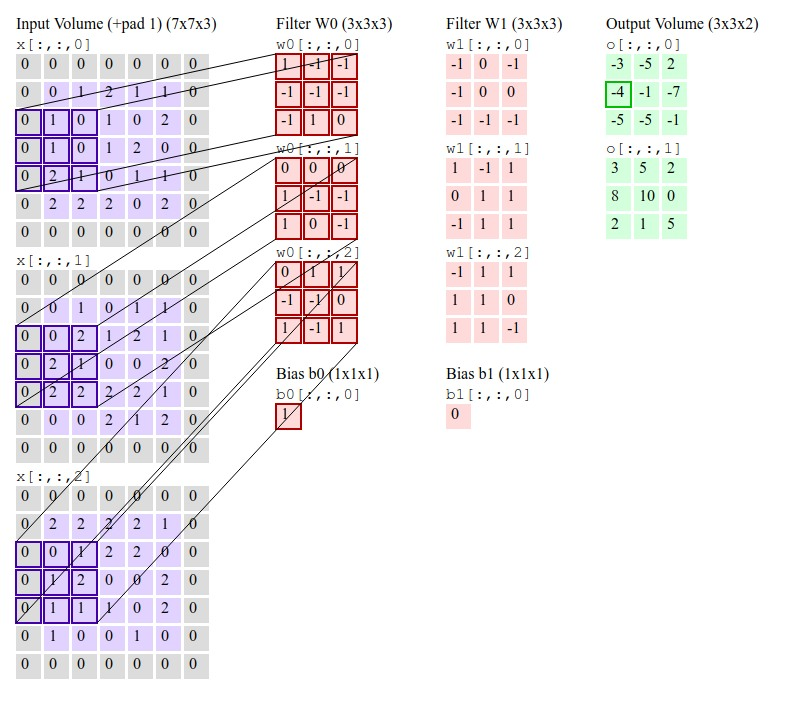
\includegraphics[scale=0.5]{{Images/chap5CNN2}.jpg}}
  \caption{Η δράση της συνέλιξης. Μια σειρά από φίλτρα κυλίονται επί της εισόδου και το αποτέλεσμα του τοπικού εσωτερικού γινομένου απεικονίζεται απευθείας στην έξοδο. Η έξοδος θα έχει διάσταση βάθους όσο και το πλήθος των φίλτρων. Οι χωρικές διαστάσεις προκύπτουν από το πλήθος των σημείων όπου υπολογίζονται τοπικά τα εσωτερικά γινόμενα καθώς το φίλτρο κυλίεται. Συνήθως, βήμα ολίσθησης μοναδιαίο σε συνδυασμό με κατάλληλη αρχική προσαύξηση με μηδενικά αφήνουν αναλλοίωτες τις χωρικές διαστάσεις εξόδου ως προς την είσοδο, ενώ η μεταβλητή είναι η διάσταση βάθους.}
  \label{fig:chap5CNN2}
\end{figure}

\par Θα αναλύσουμε σε λίγο μεγαλύτερο βάθος τη δομή ενός συνελικτικού σταδίου. Πρακτικά σε κάθε τέτοιο στάδιο η είσοδος είναι ένας όγκος $W \times H \times D$ και η έξοδος ένας νέος όγκος $W'\times H'\times D'$. Επομένως χρειάζεται να καθορίσουμε μια συνάρτηση που θα κάνει αυτόν τον μετασχηματισμό. Το στάδιο πρέπει να εφαρμόσει $N$ φίλτρα στην είσοδο. Αυτή είναι η τρίτη διάσταση της εξόδου, $D'=N$. Τώρα, κάθε νευρώνας ενός φίλτρου συνδέεται σε ένα μικρό κλάσμα της εισόδου, το λεγόμενο συναπτικό πεδίο, που καθορίζεται από τη θέση του νευρώνα στο φίλτρο. Καθώς θέλουμε θέλουμε να εφαρμόσουμε το φίλτρο σε όλη την εικόνα, έχουμε πολλούς νευρώνες ανά φίλτρο. Στην πράξη, κυλάμε το φίλτρο πάνω στην αρχική εικόνα και υπολογίζουμε το εσωτερικό γινόμενο, δηλαδή συνελίσσουμε το φίλτρο με την εικόνα, επιτρέποντας πιθανόν μετακινήσεις με μεγαλύτερο βήμα από 1. Συνοψίζοντας, νευρώνες με ίδιο μήκος και πλάτος έχουν το ίδιο συναπτικό πεδίο, ενώ νευρώνες με ίδιο βάθος είναι αντίτυπα του ίδιου φίλτρου. Κάθε φίλτρο εφαρμόζεται στο συναπτικό του πεδίο και η έξοδος αθροίζεται σε όλο το βάθος εισόδου αποδίδοντας μια τιμή εξόδου. Η σύμπτυξη αυτών των εξόδων δημιουργεί τον $W'\times H'\times D'$ χώρο εξόδου.

\subsection{Το Δίκτυο ResNet}
Το 2015, στο \cite{he_2015} εισήχθη μια νέα διάταξη των επιπέδων εντός του συνελικτικού δικτύου. Παρατηρήθηκε ότι αναδιατάσσοντας τις συνδέσεις μεταξύ των επιπέδων, τα στάδια ωθούνται στο να μαθαίνουν συναρτήσεις “υπολοίπου” (residual functions) με αναφορά στην είσοδο, της μορφής $F(x)+x$ και ότι τα δίκτυα αυτής της μορφής εκπαιδεύονται ευκολότερα, μπορούν να είναι πολύ βαθύτερα και πετυχαίνουν πολύ μεγαλύτερη ακρίβεια. Το προκύπτον δίκτυο ονομάστηκε ResNet από τη μορφή των συναρτήσεών του, που είχαν την residual μορφή.

\begin{figure}
  \centering
  \noindent\makebox[\textwidth]{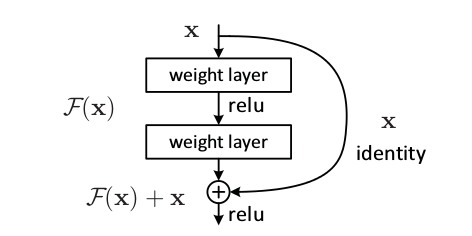
\includegraphics[scale=0.5]{{Images/chap5Res}.jpg}}
  \caption{Η μορφή των residual συναρτήσεων. Ένας εμπροσθόδρομος βρόχος παρακάμπτει ενδιάμεσα στάδια και αθροίζεται στην έξοδό τους. Το σχήμα αυτό κρύβει την πεμπτουσία των δικτύων ResNet, τα οποία βελτιστοποιούνται και πετυχαίνουν κορυφαίες αποδόσεις, ακόμα και συγκρινόμενα με άλλα συστήματα. Εικόνα από \cite{he_2015}}
  \label{fig:chap5Res}
\end{figure}

\par Η ιδέα του ResNet εκκινεί από την παρατήρηση ότι παρότι το βάθος των συνελικτικών δικτύων φαίνεται να συνεισφέρει σημαντικά στην ακρίβεια που επιτυγχάνουν, τελικά η απόδοσή τους φτάνει σε κορεσμό και περαιτέρω αύξηση του βάθους συνεισφέρει αρνητικά στην ακρίβεια καθώς δυσκολεύει πολύ η βελτιστοποίηση (degradation problem). Οι residual τοπολογίες φαίνεται να λύνουν αυτό το πρόβλημα: η τοπολογία βελτιστοποιείται εύκολα με μεθόδους Βαθμωτής Κατάβασης (Stochastic Gradient Descend) και βάθος, ακόμα και 10 φορές μεγαλύτερο είναι εφικτό, ενώ η απόδοσή τους είναι ολοένα και μεγαλύτερη. Η εξήγηση για αυτό, είναι η αρχικοποίηση προς το ταυτοτικό ταίριασμα (identity mapping). Δηλαδή, προσεγγίζοντας την $H(x)-x$, είναι ευκολότερο να επιτευχθεί σύγκλιση αν αυτό είναι βέλτιστο. Η επιτυχία του ResNet δικαιώνει πειραματικά μια τέτοια σχεδίαση, χωρίς ωστόσο απόδειξη βελτιστότητας.

\subsection{Συνελικτικά Χαρακτηριστικά και Μεταβατική Εκμάθηση (Transfer Learning)}
Η επιτυχία των νευρωνικών δικτύων έχει ωθήσει στην ευρεία χρήση τους. Εν τούτοις η εκπαίδευσή τους είναι δύσκολη και χρονοβόρα. Αυτό που είναι ενθαρρυντικό είναι η εύκολη προσαρμογή τους σε νέα καθήκοντα και σύνολα δεδομένων. Ένα βαθύ νευρωνικό δίκτυο, προεκπαιδευμένο σε κάποιο σύνολο δεδομένων, μπορεί να χρησιμοποιηθεί ως αρχικοποίηση για ένα νέο δίκτυο σε ένα νεο σύνολο δεδομένων. Ακόμα πιο ενθαρρυντικό: τα πρώτα στάδια των δικτύων σε παρόμοια καθήκοντα κωδικοποιούν πληροφορία χαμηλού επιπέδου και ελάχιστα μεταβάλλονται ανά σύνολο δεδομένων. Επομένως, αρχικοποιώντας ένα βαθύ δίκτυο με τα βάρη ενός προεκπαιδευμένου, μπορούμε να επανεκπαιδεύσουμε μόνο το τελευταίο στάδιο και να το προσαρμόσουμε στα νέα δεδομένα με επιτυχία. Μάλιστα πειράματα δείχνουν ότι τα προεκπαιδευμένα δίκτυα επιτυγχάνουν υψηλότερες επιδόσεις από δίκτυα που εκπαιδεύονται απευθείας στα νέα δεδομένα. Η τεχνική αυτή εφαρμόζεται ευρύτατα και ονομάζεται transfer learning.

\par Μπορούμε επομένως να δούμε ένα συνελικτικό νευρωνικό δίκτυο σαν μια υπολογιστική μονάδα εξαγωγής χαρακτηριστικών μεγάλης διακριτότητας και αναπαραστικής δυνατότητας. Τα χαρακτηριστικά αυτά εισάγονται σε έναν γραμμικό ταξινομητή, το τελευταίο στάδιο του δικτύου και λαμβάνουμε τις πιθανότητες κλάσεων. Γίνεται επομένως φανερό ότι μπορούμε να αντικαταστήσουμε το στάδιο εξόδου με κάποιον άλλο ταξινομητή. Μια άλλη προσέγγιση παρουσιάζεται στο \cite{tang_2013}, όπου μελετάται η χρήση SVM loss σαν συνάρτηση κόστους του δικτύου.

\subsection{BING: Binarized Normed Gradients for Objectness Estimation}
Η έννοια του μέτρου objectness αφορά στην ύπαρξη ή μη αντικειμένου σε ένα τμήμα εικόνας. Ουσιαστικά ένα σύστημα objectness προτείνει περιοχές της εικόνας όπου υπάρχουν αντικείμενα. Η ιδιότητα αυτή είναι χρήσιμη σε ανιχνευτές παραθύρων με μέθοδο κυλιόμενου παραθύρου καθώς συρρικνώνει δραστικά την περιοχή αναζήτησης.

\begin{figure}
  \centering
  \noindent\makebox[\textwidth]{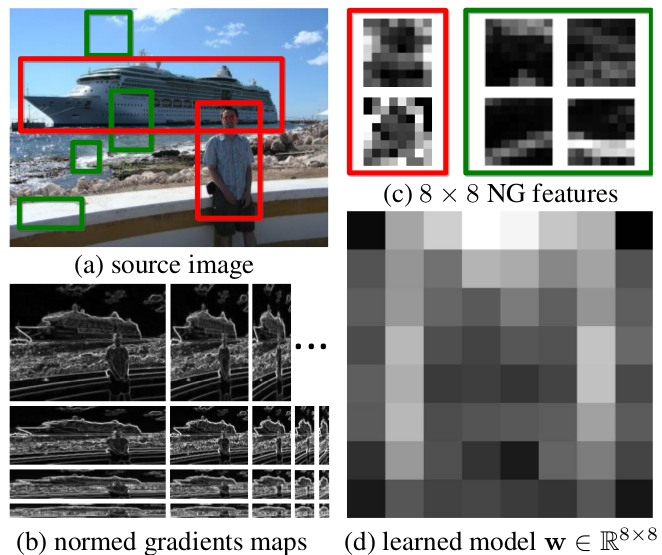
\includegraphics[scale=0.5]{{Images/chap5BING}.jpg}}
  \caption{Παρόλο που ο χώρος των παραθύρων αντικειμένων (κόκκινο) και του παρασκηνίου (πράσινο) παρουσιάζει τεράστιες διακυμάνσεις στο χώρο των εικόνων, σε κατάλληλες κλίμακες, τα κανονικοποιημένα διανύσματα παραγώγων εμφανίζουν μεγάλη συσχέτιση. Με ένα απλό μοντέλο 64 διαστάσεων, μπορούμε να λάβουμε αξιόπιστες προτάσεις για την ύπαρξη ή μη αντικειμένου. Εικόνα από \cite{cheng_2014}.}
  \label{fig:chap5BING}
\end{figure}

\par Μια γρήγορη υλοποίηση objectness προτείνεται στο \cite{cheng_2014}, όπου εισάγεται η έννοια των BING. Τα αρχικά BING μεταφράζονται σε δυαδικά κωδικοποιημένες κανονικοποιημένες παραγώγους και στηρίζονται στην παρατήρηση ότι εικόνες αντικειμένων, ανεξαρτήτως κλάσης, με ικανοποιητική ακρίβεια, μπορούν να διακριθούν από εικόνες μη αντικειμένων παρατηρώντας τις παραγώγους τους αφού προηγηθεί μια αλλαγή μεγέθους σε μια καθορισμένη τιμή. Συγκεκριμένα η αυθεντική εργασία πρότεινε το μετασχηματισμό μεγέθους σε $8 \times 8$ και τη χρήση της νόρμας των παραγώγων ως διακριτικό διάνυσμα χαρακτηριστικών 64 διαστάσεων. Εν συνεχεία, κωδικοποιούν δυαδικά τα χαρακτηριστικά αυτά ώστε να πετύχουν υψηλότερη ταχύτητα υπολογισμών με πράξεις δυαδικών τελεστών.


\section{Προτεινόμενο Σύστημα}
\subsection{Ανίχνευση Χεριών}
Για την ανίχνευση των χεριών εκπαιδεύσαμε έναν ταξινομητή κυλιόμενου παραθύρου συνδυάζοντας χαρακτηριστικά τύπου HOF, ιστογράμματα χρώματος και BING. Πιο συγκεκριμένα, χρησιμοποιήσαμε σταθερό μέγεθος παραθύρου ίσο με $31 \times 31$, οπότε τα διανύσματα HOF είχαν σταθερό μέγεθος. Για τα χαρακτηριστικά BING διατηρήσαμε τις αυθεντικές παραμέτρους και μετασχηματίζαμε κάθε παράθυρο σε εικόνα μεγέθους 8x8. Στη συνέχεια υπολογίζαμε τις παραγώγους της μετασχηματισμένης εικόνας και λαμβάνουμε τη νόρμα-1 αυτών. Τέλος, για τα ιστογράμματα χρώματος συνδυάσαμε συνιστώσες των χώρων HSV και YcbCr, επηρεασμένοι από το \cite{shaik_2015}, κρατώντας το κανάλι Η από τον πρώτο χώρο και τα κανάλια Cb, Cr από τον δεύτερο χώρο. Τα ιστογράμματα των καναλιών συνενώνονται με παράθεση (concatenation). Με ίδιο τρόπο συνενώνονται τα διαφορετικά είδη χαρακτηριστικών (HOF, BING, ιστογράμματα χρώματος). Τα χαρακτηριστικά είναι συμπληρωματικά: τα χαρακτηριστικά HOF κωδικοποιούν τη συνολική τοπική αναπαράσταση, τα ιστογράμματα χρώματος το χρώμα και τα χαρακτηριστικά BING το σχήμα.

\par Με τα χαρακτηριστικά αυτα εκπαιδεύσαμε έναν ταξινομητή Τυχαίου Δάσους (Random Forest) \cite{ho_1995}. Ο ταξινομητής αυτός δεν είναι παρά μια συλλογή δέντρων αποφάσεων όπου η τελική απόφαση προκύπτει με στάθμιση των αποφάσεων των δέντρων. Τελικά ο προκύπτων ταξινομητής είναι αποτελεσματικός αλλά και γρήγορος, καθώς οι μόνες πράξεις που έχει να εκτελέσει είναι η σύγκριση και η στάθμιση. Εκπαιδεύουμε λοιπόν έναν τέτοιο ταξινομητή σε δεδομένα τύπου “χέρι” εναντίον “όχι χέρι”. Καθώς δεν διαθέταμε σύνολο δεδομένων απόλυτα σχετικό, λάβαμε επισημειώσεις για το χέρι από ένα σύνολο \cite{rohrbach_2012}, \cite{amin_2013} που προοριζόταν για ταξινόμηση πόζας και στο οποίο η επισημείωση του χεριού ήταν σημειακή και όχι σαν περιοχή. Επιπλέον, στο σύνολο υπήρχαν εικόνες όπου το χέρι επικαλυπτόταν από άλλα αντικείμενα, εν τούτοις επισημειωνόταν. Καθαρίσαμε όσο το δυνατόν αυτές τις εικόνες. Παρείχαμε ως δεδομένα εκπαίδευσης από κάθε εικόνα τις εικόνες του χεριού, δύο εικόνες υποβάθρου και, αραιά, εικόνες κεφαλιού. Με αυτόν τον τρόπο δηλώνουμε ρητά ότι δεν αρκούν εικόνες δέρματος ως θετικά δείγματα αλλά εικόνες χεριών. Το κριτήριο βελτιστοποίησης του ταξινομητή επιλέχθηκε να είναι η μετρική Precision, καθώς θέλουμε τον λιγότερο δυνατό αριθμό εσφαλμένων θετικών εκτιμήσεων. Με cross-validation μετρήσαμε 94\% precision στη φάση εκπαίδευσης.

\begin{figure}
  \centering
  \noindent\makebox[\textwidth]{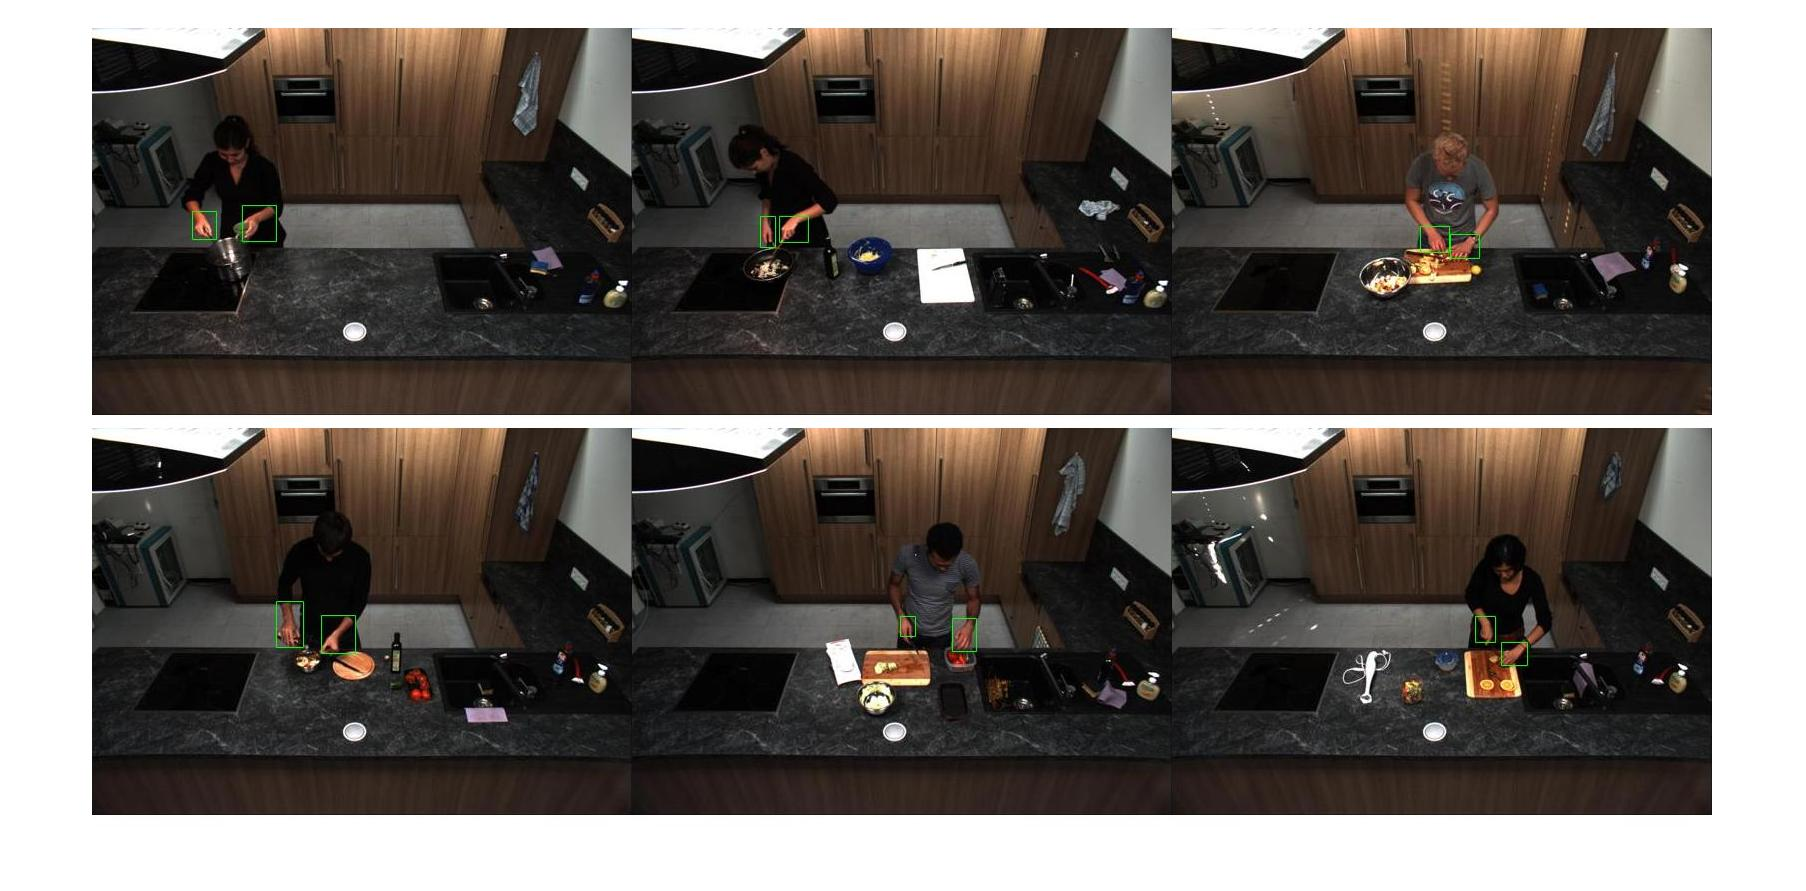
\includegraphics[scale=0.3]{{Images/chap5Success}.jpg}}
  \caption{Παραδείγματα επιτυχούς ανίχνευσης χεριών. Τα προκύπτοντα παράθυρα μπορούν να εισέλθουν στο επόμενο στάδιο εξαγωγής χαρακτηριστικών και τελικά να ταξινομηθούν ως τύποι λαβής.}
  \label{fig:chap5Success}
\end{figure}

\begin{figure}
  \centering
  \noindent\makebox[\textwidth]{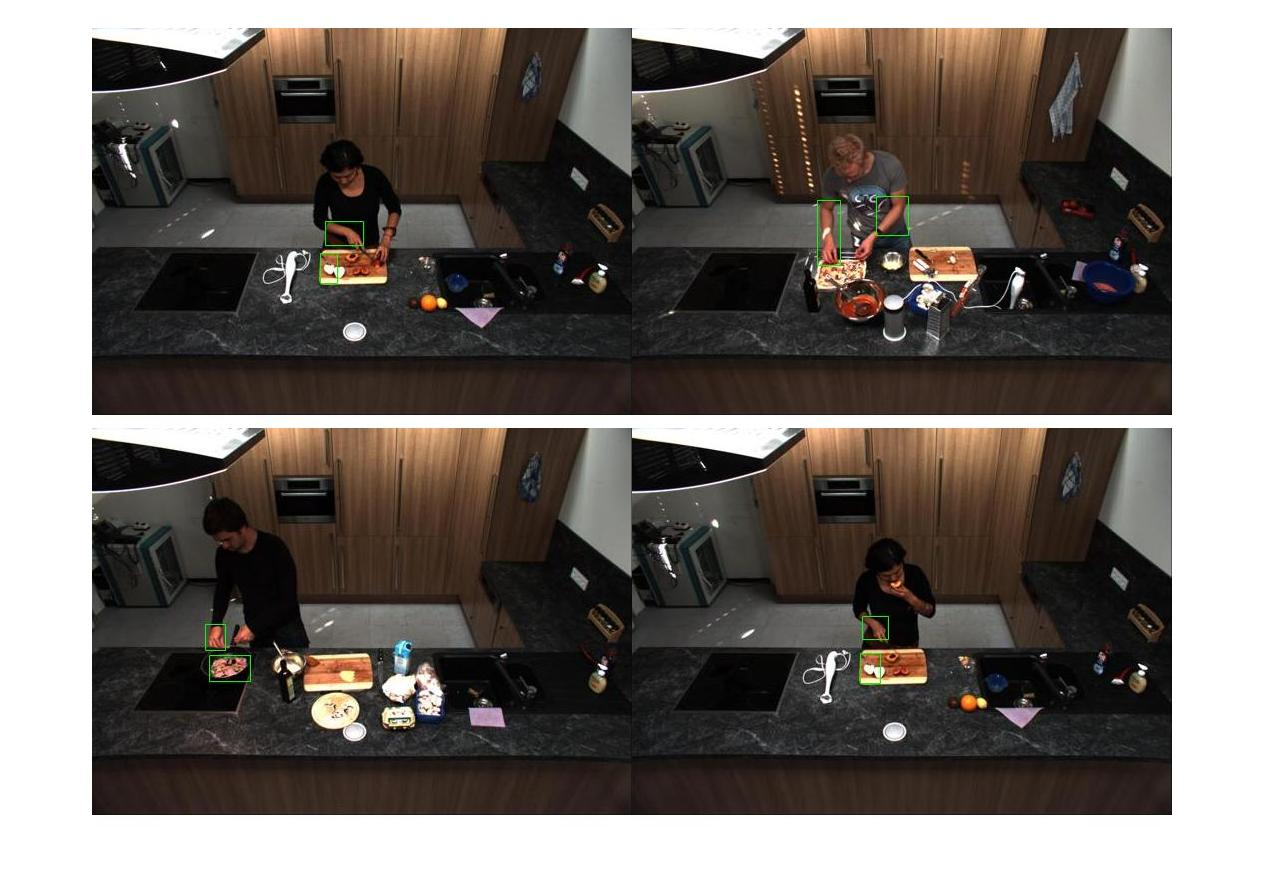
\includegraphics[scale=0.3]{{Images/chap5Failure}.jpg}}
  \caption{Περιπτώσεις όπου η ανίχνευση χεριών αποτυγχάνει. Είναι πιθανό, περιοχές κοντά σε χέρια να ταξινομηθούν ως χέρια λόγω του χρωματικού κατωφλίου και των περιορισμών έκτασης που εφαρμόζονται στο τικό στάδιο του αλγορίθμου ανίχνευσης. Εν τούτοις, προτιμήθηκε η ύπαρξη τέτοιων σφαλμάτων μπροστά στα οφέλη μιας τέτοιας σχεδίασης. Κατά την εξαγωγή του τύπου λαβής, τα σφάλματα εισάγουν θόρυβο που αντισταθμίζουμε με την εισαγωγή επιπλέον κατηγοριών στο στάδιο μη επιβλεπόμενου διαχωρισμού.}
  \label{fig:chap5Failure}
\end{figure}

\par Στη φάση ελέγχου, κυλάμε παράθυρο $31 \times 31$ πάνω στην εικόνα με βήμα 10 σε κάθε διάσταση, οπότε λαμβάνουμε επικαλυπτόμενα παράθυρα. Το βήμα επιλέχθηκε στην τιμή αυτή ως συμβιβασμός μεταξύ ακρίβειας και ταχύτητας. Για κάθε παράθυρο εξάγουμε τα χαρακτηριστικά και αφήνουμε τον ταξινομητή να αποφασίσει αν η εικόνα είναι εικόνα χεριού ή όχι. Παρότι η εκπαίδευση παρουσιάζει πολύ καλή μετρική precision, είναι φανερό ότι λόγω του μεγάλου αριθμού παραθύρων ανά εικόνα, δεν μπορούμε να αποφύγουμε την εμφάνιση εσφαλμένων θετικών εκτιμήσεων. Αντιμετωπίζουμε αυτό το φαινόμενο με επιπλέον επεξεργασία των αποτελεσμάτων σε 3 στάδια.

\par Στο πρώτο στάδιο γίνεται η εκτίμηση των superpixels \cite{srivatsa_2015}. Πρακτικά αντιστοιχίζουμε στην εικόνα έναν χάρτη πιθανοτήτων ύπαρξης χεριού. Η δημιουργία αυτού του χάρτη γίνεται ως εξής: Αρχικοποιούμε το χάρτη στο 0. Για κάθε παράθυρο που έχει ταξινομηθεί ως παράθυρο χεριού προσθέτουμε 1 στην αντίστοιχη περιοχή στο χάρτη. Τελικά κανονικοποιούμε τον προκύπτοντα χάρτη, λαμβάνοντας μια γκρίζα εικόνα όπου η τιμή κάθε pixel δηλώνει την πιθανότητα το pixel αυτό να είναι pixel χεριού. Για να λάβουμε τα superpixels χρειάζεται να μετατρέψουμε το χάρτη πιθανοτήτων σε δυαδική εικόνα. Αυτό γίνεται με τη χρηση κατωφλίου, το οποίο στην περίπτωσή μας επιλέχθηκε ίσο με 0.5. Τα superpixels είναι επομένως συμπαγείς περιοχές περιοχές pixels με ενιαία ιδιότητα, που εδώ η ταξινόμησή τους ως pixels χεριού. Η χρήση superpixels φιλτράρει επιπλέον τις λανθασμένες θετικές ταξινομήσεις στην περίπτωση που δεν έχουν ισχυρή γειτονιά, δηλαδή γειτονικές περιοχές χεριού.

\begin{figure}
  \centering
  \noindent\makebox[\textwidth]{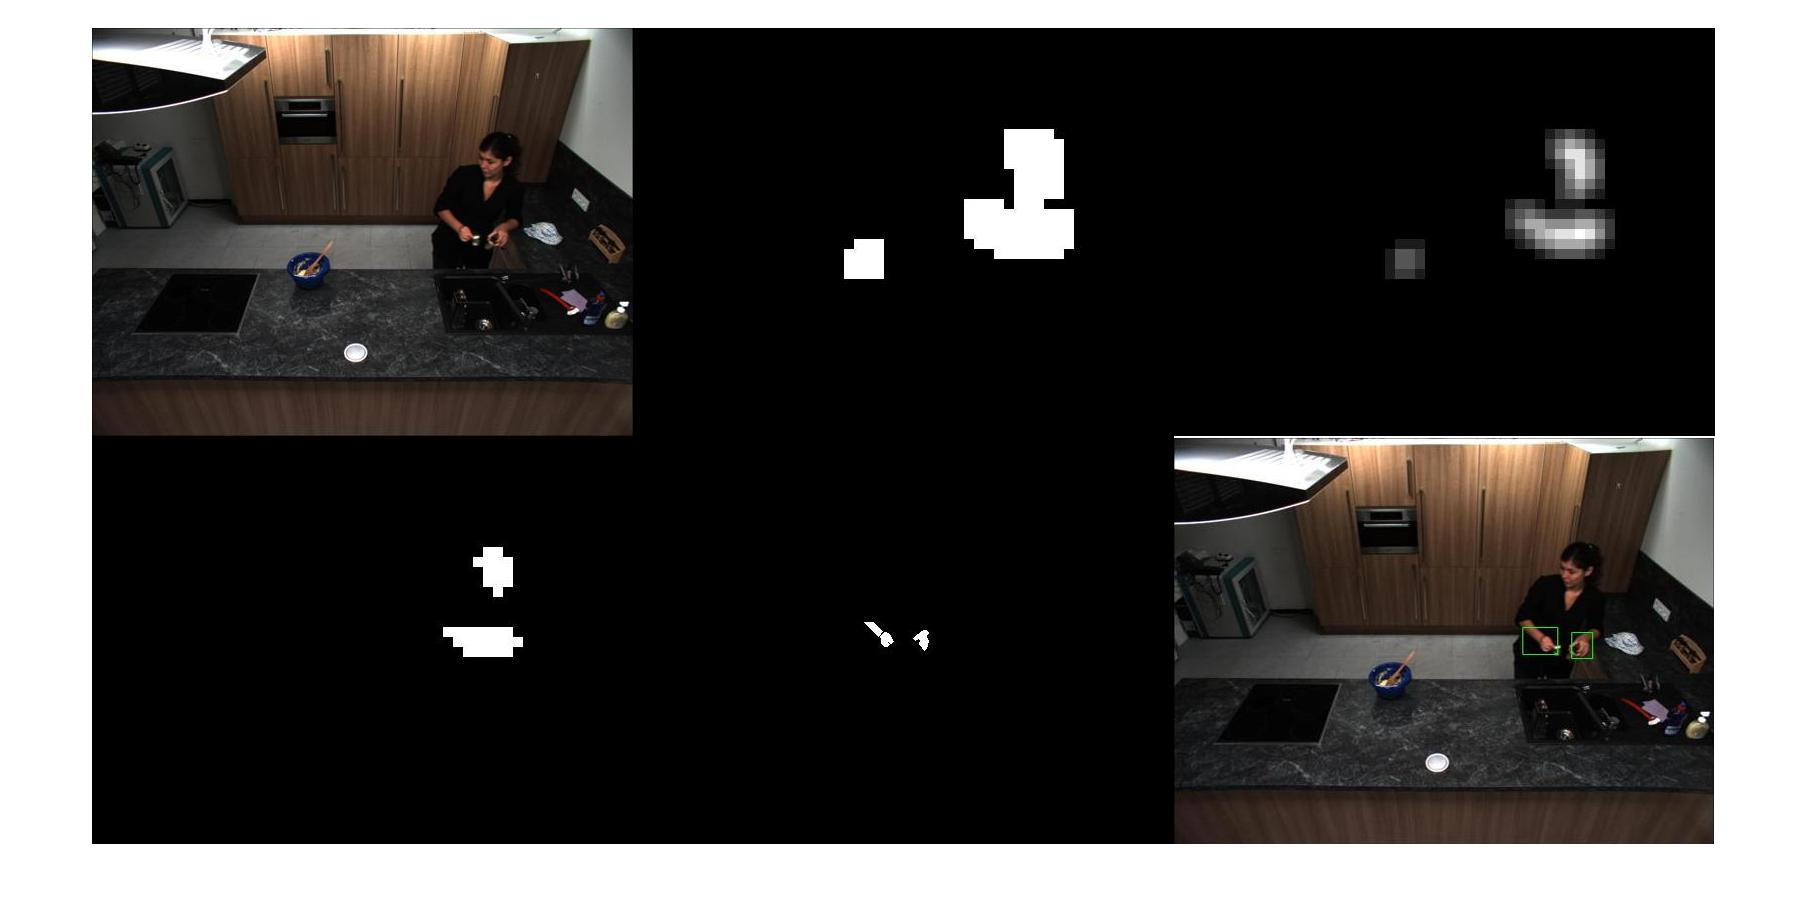
\includegraphics[scale=0.25]{{Images/chap5Steps}.jpg}}
  \caption{Βήματα του αλγορίθμου ανίχνευσης χεριών. Η αρίθμηση εφαρμόζεται από πάνω αριστερά προς τα κάτω δεξιά. \textbf{Εικόνα 1:} Η αρχική εικόνα. \textbf{Εικόνα 2:} Η περιοχή που καλύπτουν τα παράθυρα με μηδενική πιθανότητα συμπερίληψης χεριού. Τα παράθυρα αυτά προκύπτουν από την κύλιση ενός παραθύρου πάνω στην εικόνα, την εξαγωγή τοπικών χαρακτηριστικών και την ταξινόμηση αυτών. \textbf{Εικόνα 3:} Ο χάρτης πιθανοτήτων ύπαρξης χεριού. Ο χάρτης αυτός προκύπτει μετά από κανονικοποίηση της εικόνας 2. \textbf{Εικόνα 4:} Τα superpixels. Ο χάρτης των superpixels προκύπτει από την κατωφλίωση του χάρτη πιθανοτήτων. Βλέπουμε ότι υπάρχουν δύο συμπαγείς περιοχές πλέον. Καθώς στο άξονα $y$ δεν υπάρχει επικάλυψη, η πάνω περιοχή αποκόπτεται. Η κάτω περιοχή χρειάζεται επιπλέον ανάλυση για διαχωρισμό των χεριών. \textbf{Εικόνα 5:} Με την εφαρμογή χρωματικών κατωφλίων και μορφολογικών τελεστών απομονώνουμε τις περιοχές των χεριών. \textbf{Εικόνα 6:} Η τελική εικόνα ανίχνευσης.}
  \label{fig:chap5Steps}
\end{figure}

\par Στο δεύτερο στάδιο υπολογίζουμε τα κουτιά των διακριτών superpixels και λαμβάνουμε μια εκτίμηση του εμβαδού τους. Κρατάμε το πολύ 3 κουτιά, αυτά με το μεγαλύτερο εμβαδόν, με την περίπτωση των τριών κουτιών να συμβαίνει μόνο όταν υπάρχει ισοβαθμία εμβαδών. Υποθέτουμε ότι τα χέρια θα είναι σε παρόμοιο ύψος, οπότε θα υπάρχει μια οριζόντια ευθεία η θα διέρχεται μέσα από όλα τα κουτιά χεριών. Αν δεν υπάρχει τέτοια ευθεία, κρατάμε μόνο τα κουτιά για τα οποία μπορεί να βρεθεί οριζόντια ευθεία η οποία να διέρχεται από μέσα από τα ίδια και το χαμηλότερο σε ύψος κουτί. Η επιλογή αυτή γίνεται ώστε να κόψει εσφαλμένα θετικά κουτιά στην περιοχή του κεφαλιού. Τέλος, απορρίπτονται τα κουτιά με εμβαδόν μικρότερο των 300 τετραγωνικών pixels, εκτός αν αυτό αποτελεί το μέγιστο εμβαδόν περιοχής χεριού από αυτές που ανιχνεύθηκαν.

\par Στο τρίτο στάδιο, διαχωρίζονται οι περιοχές που έχουν μείνει σε υποπεριοχές μεγαλύτερης ακριβείας. Το κίνητρο πίσω από αυτό είναι ότι συχνά τα δύο χέρια βρίσκονται κοντά μεταξύ τους οπότε οι περιοχές τους επικαλύπτονται στα superpixels και προκύπτει μία περιοχή μόνο και για τα δύο χέρια. Ο επιπλέον διαχωρισμός γίνεται με κατανομή χρώματος. Ο αλγόριθμος βασίζεται στο \cite{kolkur_2016} και αξιοποιεί την χρωματική πληροφορία των χώρων RGB, HSV και YCbCr. Σύμφωνα με την εργασία αυτή, ικανοποιητική χρωματική συνθήκη για δέρμα είναι η 

\begin{equation}\label{eq:ColorSpace}
\begin{gathered}
    \big( (R>95) \cap (G>40) \cap (B>20) \cap (R>G) \cap (R>B) \cap (| R-G |>15) \cap (A>15) \big) \\ \cap \\ \bigg( \big( (0\leq H\leq 50) \cap (0.23\leq S\leq 0.68) \big) \\ \cup \\ \big( (Cr>135) \cap (Cb>85) \cap (Y>80) \\ \cap (Cr\leq (1.5862Cb)+20) \\ \cap (Cr\geq 0.3448Cb+76.2069) \\ \cap (Cr\leq -4.5652Cb+234.5652) \\ \cap (Cr\leq -1.15Cb+301.75) \\ \cap (Cr\leq -2.2857Cb+432.85) \big) \bigg)
\end{gathered}
\end{equation}

\par Εφαρμόζουμε αυτή τη συνθήκη για να παράγουμε δυαδικές εικόνες από κάθε superpixel χεριού. Για να κόψουμε το θόρυβο εφαρμόζουμε μορφολογικό opening με κύκλο ακτίνας 2. Αν αυτό κόβει όλη την εικόνα, χρησιμοποιούμε κύκλο ακτίνας 1. Αν και αυτό κόβει όλη την εικόνα, εφαρμόζουμε closing με κύκλο ακτίνας 2. Η τελευταία περίπτωση λειτουργεί στην εμφάνιση χεριών υπό γωνία τέτοια ώστε να φαίνεται μικρό μέρος τους. Υπολογίζουμε τα νέα superpixels και κρατάμε και πάλι το πολύ 3 περιοχές, τις μεγαλύτερες σε εμβαδόν. Κόβουμε όλες τις περιοχές με εμβαδόν μικρότερο του 99. Με αυτόν τον τρόπο πετάμε αρκετό θόρυβο και διαχωρίζουμε τα χέρια τα οποία αρχικά βρίσκονταν εντός του ίδιου superpixel. Ακολουθεί ένα τελικό στάδιο στο οποίο κρατάμε τα δύο (αν υπάρχουν) μεγαλύτερα σε εμβαδόν superpixels από την ένωση όλων των περιοχών και επιστρέφουμε αυτά ως τελικές περιοχές χεριών.

\subsection{Εξαγωγή Τύπου Λαβής}
Ο τύπος λαβής μπορεί να περιέχει πληροφορία για τη χρήση των σχετιζόμενων με τη δράση αντικειμένων και τελικά με την ίδια τη δράση. Πειράματα στο \cite{zhang_2015} δείχνουν την αξία του τύπου λαβής στην αναγνώριση του σκοπού του χειριστή αντικειμένων. Επιπλέον, αποτελούν και χαρακτηριστικά χρήσιμα στην κατάτμηση του βίντεο σε δράσεις. Στο \cite{yang_2015_grasp} παρουσιάζεται μια χρήσιμη ταξινόμηση τύπων λαβής για πλούσια πληροφορία σχετικά με την αναγνώριση δράσης και σκοπού. Η ταξινόμηση αυτή εστιάζει στη λειτουργικότητα και χωρίζει τις  λαβές σε τρεις μεγάλες κατηγορίες: προσανατολισμένες σε δύναμη, σε ικανότητα και καθημερινές. Η ταξινόμηση αυτή είναι παρόμοια με την πιο γενική, η οποία διαχωρίζει σε λαβές δύναμης, ακριβείας και έκταση/ξεκούραση. Εδώ διαχωρίζουμε επιπλέον τις λαβές δύναμης σε κυλινδρικές, σφαιρικές και σε μορφή γάντζου, ενώ επίσης διαχωρίζουμε τις λαβές ακριβείας σε τσιμπήματος, τριποδικές και παράδοσης (lumbrical). Οπότε μαζί με τις περιπτώσεις έκτασης και ξεκούρασης, όπου δεν πραγματοποιείται κάποια λαβή από τις παραπάνω, έχουμε 8 κατηγορίες λαβών.

\begin{figure}
  \centering
  \noindent\makebox[\textwidth]{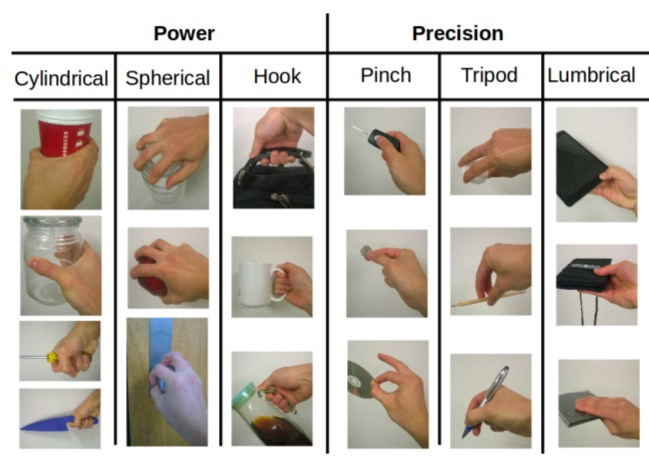
\includegraphics[scale=0.5]{{Images/chap5GraspTypes}.jpg}}
  \caption{Οι τύποι λαβής στους οποίους στηριζόμαστε ως χρήσιμη πληροφορία για την αναγνώριση δράσεων. Λαβές που δεν ταξινομούνται σε αυτές τις κατηγορίες θα είναι λαβές έκτασης και ξεκούρασης. Εικόνα από \cite{yang_2015_grasp}.}
  \label{fig:chap5GraspTypes}
\end{figure}

\par Για την αναγνώριση του τύπου λαβών δεν διαθέτουμε κάποιο σύνολο δεδομένων που να μπορεί να προσαρμοστεί στα δικά μας δεδομένα, οπότε αναγκαστήκαμε να κινηθούμε με μη επιβλεπόμενη μάθηση. Συγκεκριμένα, σε πρώτη φάση υπολογίζουμε τα συνελικτικά χαρακτηριστικά για τις εικόνες χεριών που εντοπίζονται αυτόματα στα βίντεο εκπαίδευσης, χρησιμοποιώντας το ResNet. Στη συνέχεια χρησιμοποιούμε τη μέθοδο των k-μέσων για να εξάγουμε 10 κέντρα κατηγοριών. Επιλέξαμε 10 κέντρα αντί για 8 ώστε να κόψουμε περιπτώσεις θορύβου από την ανίχνευση χεριών, καθώς δεν υπάρχει Ground Truth επισημείωση. Λαμβάνοντας τα 10 κέντρα, εκπαιδεύουμε και εφαρμόζουμε ταξινόμηση με χρήση του αλγορίθμου Στοχαστικής Βαθμωτής Κατάβασης (Stochastic Gradient Denscend, SGD) στα δείγματα εκπαίδευσης και δημιουργούμε τα ιστογράμματα τύπων λαβής για τα δεδομένα εκπαίδευσης. Να σημειωθεί ότι σε κάθε frame που εξετάζουμε, θα εμφανίζονται το πολύ δύο χέρια, ωστόσο δεν είναι εκ των προτέρων γνωστό το ποιο από τα δύο θα εμφανίζεται ή ποιο από τα δύο χέρια αντιστοιχεί στο αριστερό και ποιο στο δεξί. Οπότε αθροίζουμε τα ιστογράμματα για τα δύο χέρια που εμφανίζονται, εκμεταλλευόμενοι την προσεταιριστική ιδιότητα. Αν εμφανίζεται μόνο ένα χέρι στο frame τότε το δεύτερο διάνυσμα είναι το μηδενικό διάνυσμα 10 διαστάσεων. Εφαρμόζουμε την ίδια διαδικασία στα δείγματα εκπαίδευσης για να λάβουμε τα ιστογράμματα εκπαίδευσης. Στο κεφάλαιο 6 θα δείξουμε πώς συνενώνουμε αυτά τα χαρακτηριστικά και τη συνεισφορά τους στην ταξινόμηση.



\end{document}
